\documentclass[letterpaper]{article}
\usepackage[margin=1in]{geometry}
\usepackage[utf8]{inputenc}
\usepackage{textcomp}
\usepackage{amssymb}
\usepackage{natbib}
\usepackage{graphicx}
\usepackage{gensymb}
\usepackage{amsthm, amsmath, mathtools}
\usepackage[dvipsnames]{xcolor}
\usepackage{enumerate}
\usepackage{mdframed}
\usepackage[most]{tcolorbox}
\usepackage{csquotes}
% https://tex.stackexchange.com/questions/13506/how-to-continue-the-framed-text-box-on-multiple-pages

\tcbuselibrary{theorems}

\newcommand{\R}{\mathbb{R}}
\newcommand{\Z}{\mathbb{Z}}
\newcommand{\N}{\mathbb{N}}
\newcommand{\Q}{\mathbb{Q}}
\newcommand{\C}{\mathbb{C}}
\newcommand{\code}[1]{\texttt{#1}}
\newcommand{\mdiamond}{$\diamondsuit$}
\newcommand{\PowerSet}{\mathcal{P}}
\newcommand{\Mod}[1]{\ (\mathrm{mod}\ #1)}
\DeclareMathOperator{\lcm}{lcm}

%\newtheorem*{theorem}{Theorem}
%\newtheorem*{definition}{Definition}
%\newtheorem*{corollary}{Corollary}
%\newtheorem*{lemma}{Lemma}
\newtheorem*{proposition}{Proposition}


\newtcbtheorem[number within=section]{theorem}{Theorem}
{colback=green!5,colframe=green!35!black,fonttitle=\bfseries}{th}

\newtcbtheorem[number within=section]{definition}{Definition}
{colback=blue!5,colframe=blue!35!black,fonttitle=\bfseries}{def}

\newtcbtheorem[number within=section]{corollary}{Corollary}
{colback=yellow!5,colframe=yellow!35!black,fonttitle=\bfseries}{cor}

\newtcbtheorem[number within=section]{lemma}{Lemma}
{colback=red!5,colframe=red!35!black,fonttitle=\bfseries}{lem}

\newtcbtheorem[number within=section]{example}{Example}
{colback=white!5,colframe=white!35!black,fonttitle=\bfseries}{def}

\newtcbtheorem[number within=section]{note}{Important Note}{
        enhanced,
        sharp corners,
        attach boxed title to top left={
            xshift=-1mm,
            yshift=-5mm,
            yshifttext=-1mm
        },
        top=1.5em,
        colback=white,
        colframe=black,
        fonttitle=\bfseries,
        boxed title style={
            sharp corners,
            size=small,
            colback=red!75!black,
            colframe=red!75!black,
        } 
    }{impnote}
\usepackage[utf8]{inputenc}
\usepackage[english]{babel}
\usepackage{fancyhdr}
\usepackage[hidelinks]{hyperref}

\pagestyle{fancy}
\fancyhf{}
\rhead{MATH 180A}
\chead{Friday, April 29, 2022}
\lhead{Lecture 14}
\rfoot{\thepage}

\setlength{\parindent}{0pt}

\begin{document}

\section{Expected Value and Variance}
Let $X$ be a continuous (potentially very complicated) random variable with PDF $f$. Suppose we were asked to pick \emph{one real number} $\mu$, subject to a certain constraint, that best represents the random variable $X$. Of course, note that $X$ is a random variable and might be very different than just one single (deterministic) real number. That being said, we want to try our best to pick said real number that satisfies this constraint.

\subsection{Expected Value}
One natural thing to do is to pick a $\mu$ so that best represents the random variable (i.e., is closest to the random variable). So, we can consider the \emph{squared distance}. In particular, we want to find a $\mu$ such that \[(X - \mu)^2\] is likely to be as close to 0 as possible. Note that $(X - \mu)^2$ is itself a random variable. Put it another way, we want to find a $\mu$ that minimize the random distance $(X - \mu)^2$. So, we want to minimize 
\[\int_{-\infty}^{\infty} (x - \mu)^2 f(x) dx.\]
By linearity, we have 
\begin{equation*}
    \begin{aligned}
        \int_{-\infty}^{\infty} (x - \mu)^2 f(x) dx &= \int_{-\infty}^{\infty} (x^2 - 2x\mu + \mu^2) f(x) dx \\ 
            &= \int_{-\infty}^{\infty} x^2 f(x) dx - 2\mu \int_{-\infty}^{\infty} xf(x) dx + \mu^2 \int_{-\infty}^{\infty} f(x) dx. 
    \end{aligned}
\end{equation*} 
Since $f(x)$ is a PDF, the third integral is just 1. Hence, we want to minimize 
\[\int_{-\infty}^{\infty} x^2 f(x) dx - 2\mu \int_{-\infty}^{\infty} xf(x) dx + \mu^2.\]
Differentiating with respect to $\mu$, we get 
\[-2 \int_{\infty}^{\infty} xf(x) dx + 2\mu.\]
If we set this equal to 0 and then solve for $\mu$, we find the minimizer is 
\[\mu = \int_{-\infty}^{\infty} xf(x) dx.\]
We note that $\mu$ is a \textbf{weighted average}. We integrate over all possible values of $x$, and then weigh them by their corresponding density $f(x)$. 

\begin{definition}{Expected Value}{}
    Suppose that $X$ is a continuous random variable with PDF $f$. Then, the \textbf{expected value} (or \textbf{mean}) of $X$ is 
    \[\mu = \mathbb{E}(X) = \int_{-\infty}^{\infty} xf(x)dx.\]
\end{definition}
\textbf{Remarks:} 
\begin{itemize}
    \item For some random variables, this expected value (integral) does not exist. We won't need to worry about this here, though. 
    \item If $X$ is a \textbf{discrete} random variable with PMF $p(x) = \PR(X = x)$, then $\mu = \mathbb{E}(X) = \sum_{x} xp(x)$. 
\end{itemize}
The \textbf{mean} $\mu$ gives us valuable information about the ``center'' of a distribution. This, along with \textbf{standard deviation} $\mu$ (which tells us about the ``spread'' of a distribution), tells us the fundamental quantities in regards to the ``shape'' of a distribution. 

\begin{mdframed}[]
    (Example.) Suppose we roll a fair die, which takes values between 1 and 6, each with equal probability $\frac{1}{6}$. Then, 
    \[\mu = \sum_{k = 1}^{6} k \cdot \frac{1}{6} = \frac{1}{6} \sum_{k = 1}^{6} k = \frac{7}{2}.\]
    Here, we're considering all possible values that the die can take (from $k = 1$ to 6). Each value has a probability of $\frac{1}{6}$. 

    \bigskip 

    While $\frac{7}{2}$ is not a value that the random variable can actually take (note that the random variable can only take values 1, 2, 3, 4, 5, and 6), but in some sense it is the expected value, or the average value. To see why this is the case, consider the following histogram:  
    \begin{center}
        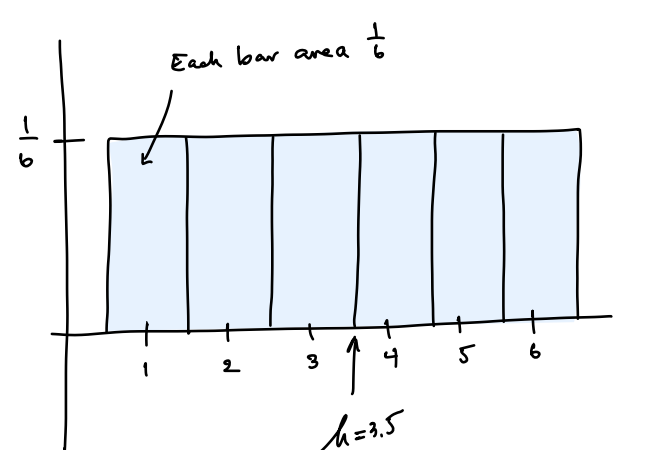
\includegraphics[scale=0.7]{../assets/lec14die.png}
    \end{center} 
    We can think of the 3.5 mark as the ``center of mass.''
\end{mdframed}

\begin{theorem}{Law of Unconscious Statistics (LotUS)}{}
    Suppose that $X$ is a random variable and $\phi: \R \mapsto \R$ is a function. Then, 
    \begin{enumerate}
        \item If $X$ is continuous with PDF $f$, then 
        \[\mathbb{E}[\phi(X)] = \int_{-\infty}^{\infty} \phi(x) f(x) dx.\]

        \item If $X$ is discrete with PMF $p$, then 
        \[\mathbb{E}[\phi(X)] = \sum_{x} \phi(x) p(x).\]
    \end{enumerate}
\end{theorem}
\textbf{Remarks:} 
\begin{itemize}
    \item It is enough \emph{just} to know the PDF/PMF of $X$ to find the expected value of $Y = \phi(X)$.
    \item This shows us that expectation is linear. In particular, the \textbf{Linearity of Expectation} (LoE) says that if we let $X$ be a random variable, then we can suppose that $a, b \in \R$. Then, $\mathbb{E}(aX + b) = a\mathbb{E}(X) + b$. 
\end{itemize}
\textbf{Warning:}
\begin{itemize}
    \item LoE does not imply that $\mathbb{E}(XY) = \mathbb{E}(X) \mathbb{E}(Y)$. 
    \item Note that this is true if $X$ and $Y$ are independent, but not true otherwise. 
\end{itemize}

\subsection{Variance}
\begin{definition}{Variance}{}
    The \textbf{variance} of a random variable $X$, denoted by $\sigma^2 = \text{Var}(X)$, is the expected squared distance of $X$ from its mean $\mu$. That is, $\sigma^2 = \mathbb{E}[(X - \mu)^2]$. 
\end{definition}
\textbf{Remarks:}
\begin{itemize}
    \item This is telling us about the \emph{spread} of the distribution; that is, how far away should we expect the random variable to be away from its mean. 
    \item Recall that the mean $\mu$ is the real number that minimizes $\mathbb{E}[(X - a)^2]$ over all real numbers $a$. Whatever this quantity happens to be at the minimizer $a = \mu$ is called the variance $\sigma^2$. 
\end{itemize}

\begin{theorem}{}{}
    Let $X$ be a random variable and let $a, b \in \R$. Then, 
    \[\text{Var}(aX + b) = a^2\text{Var}(X) = a^2 \mathbb{E}[(X - \mu)^2].\]
\end{theorem}
\textbf{Remark:} Note that the variance of a constant is 0, since the distribution of a constant random variable has no ``spread'' at all. 

\textbf{Warning:} While expected value is linear, variance is not. In other words, if $X$ and $Y$ are \emph{independent}, then $\text{Var}(X + Y) = \text{Var}(X) + \text{Var}(\text{Y})$. However, this is not true in general. 

\bigskip 

Note that the formula $\sigma^2 = \mathbb{E}[(X - \mu)^2]$ is useful conceptually, but not so convenient for computations. Instead, we can use the Linearity of Expectation to obtain the following, more convenient, formula: 
\[\sigma^2 = \mathbb{E}(X^2 - 2\mu X + \mu^2) = \mathbb{E}(X^2) - 2\mu \mu + \mu^2 = \mathbb{E}(X^2) - \mu^2.\]
Therefore, the \textbf{computational variance formula} is given by 
\[\boxed{\text{Var}(X) = \mathbb{E}(X^2) - [\mathbb{E}(X)]^2}.\]
The quantity $\mathbb{E}(X^2)$ is called the \textbf{second moment} of $X$, and can be computed using LotUS. That is, if $X$ is continuous, then 
\[\mathbb{E}(X^2) = \int_{-\infty}^{\infty} x^2 f(x) dx.\]
If $X$ is discrete, then 
\[\mathbb{E}(X^2) = \sum_{x} x^2 p(x).\]

\subsection{Standard Deviation}
\begin{definition}{Standard Deviation}{}
    The square root of the variance, $\sigma = \sqrt{\text{Var}(X)}$, is called the \textbf{standard deviation} of $X$.
\end{definition}
The reason for the name is that, for ``most reasonable'' distributions, the ``bulk'' of the mass/density deviates by at most $\sigma$ from the center $\mu$. That is, usually, ``most'' of the mass/density is on the values of 
\[x \in [\mu - \sigma, \mu + \sigma].\]

\begin{theorem}{Chebyshev's Inequality}{}
    Let $X$ be a random variable with \emph{both} mean $\mu$ and standard deviation $\sigma$. Then, for any real number $a > 0$, we have that 
    \[\PR(|X - \mu| \geq a \sigma) \leq \frac{1}{a^2}.\]
\end{theorem}
\textbf{Remarks:}
\begin{itemize}
    \item In other words, for any distribution with a mean and variance, the probability that $X$ is at least $a = 2$ standard deviations from the center $\mu$ of the distribution is at most $\frac{1}{4}$.
    \item For many distributions, the actual probability is \emph{much} smaller. However, this is an useful upper bound that works for all distributions.
\end{itemize}
This result follows by 
\begin{theorem}{Markov's Inequality}{}
    Let $X$ be a non-negative random variable, i.e. $\PR(X \geq 0) = 1$, with mean $\mu$ and $b > 0$ a positive number. Then, $\PR(X \geq b) \leq \frac{\mu}{b}$. 
\end{theorem}

\begin{mdframed}[]
    \begin{proof}
        (Continuous Case.) Since $X$ is non-negative, we know that 
        \[\mu = \int_{-\infty}^{\infty} xf(x) dx = \int_0^{\infty} xf(x) dx.\]
        Splitting the integral, we have 
        \[\int_{0}^{b} xf(x) dx + \int_{b}^{\infty} xf(x) dx \geq \int_{b}^{\infty} xf(x) dx \geq b \int_{b}^{\infty} f(x) dx = b \PR(X \geq b).\]
        Hence, $\PR(X \geq b) \leq \frac{\mu}{b}$, as claimed.
    \end{proof}
\end{mdframed}

\end{document}